\documentclass{article}

\PassOptionsToPackage{numbers, compress}{natbib}
\usepackage[main, final]{neurips_2026}

\usepackage[utf8]{inputenc} % allow utf-8 input
\usepackage[T1]{fontenc}    % use 8-bit T1 fonts
\usepackage{hyperref}       % hyperlinks
\usepackage{url}            % simple URL typesetting
\usepackage{booktabs}       % professional-quality tables
\usepackage{amsfonts}       % blackboard math symbols
\usepackage{nicefrac}       % compact symbols for 1/2, etc.
\usepackage{microtype}      % microtypography
\usepackage{xcolor}         % colors
\usepackage{graphicx}
\usepackage{amsmath}

% Placeholder for Connor's parts; delete the macro once they are filled in.
\newcommand{\connor}[1]{\textcolor{red}{[Connor: #1]}}

\title{Which Surrogates Matter? What Drives Success in\\Ensemble Transfer Attacks}

\author{%
  Connor Kilrain \And Mo Liu
}

\begin{document}

\maketitle

\begin{abstract}
  Transfer attacks craft adversarial examples on an ensemble of public ``surrogate'' models in the hope that they also fool an unseen target, yet surrogates are usually picked ad hoc. We study what drives the success of such ensemble attacks on ImageNet classifiers, each team member examining a different driver on a shared pipeline. One direction uses Shapley values to measure how much each surrogate, and each pair of surrogates, contributes to fooling held-out targets. \connor{one sentence on your direction.}
\end{abstract}

\section{Problem Definition}

\textbf{Setting.} An attacker wants to fool a deployed image classifier (the \emph{target}) whose weights and gradients are hidden. In a \emph{transfer attack}, the attacker crafts a small perturbation against public white-box \emph{surrogate} models and hopes it transfers. Attacking an ensemble of surrogates at once transfers far better than attacking a single one \citep{liu2017delving, dong2018boosting}.

\textbf{Problem and motivation.} Which surrogates belong in the ensemble, and why? Surrogates are not interchangeable: their gradients often conflict \citep{liu2017delving, xiong2022svre}, adversarial examples transfer poorly between CNNs and Vision Transformers \citep{mahmood2021robustness}, and each extra surrogate adds a forward and backward pass at every attack step. Knowing which public models make potent surrogates tells model owners how exposed a deployed model is, makes red-teaming cheaper, and explains \emph{why} ensemble attacks work.

\textbf{Goal.} We aim to understand what makes an ensemble of surrogates transfer well; we share one attack pipeline, model pool, and metric, each study a different angle, and synthesize our findings. Mo's direction asks: \emph{how much does each surrogate, and each pair of surrogates, contribute to an ensemble attack's success on unseen targets?} We hypothesize that a surrogate's value in an ensemble depends more on what it adds to the others than on its standalone strength, so ranking surrogates by Shapley value will differ noticeably from ranking them by how well each transfers alone. \connor{your research question(s).}

\section{Relevance to Trustworthy Aspects}

\textbf{Adversarial robustness (primary):} we \emph{evaluate} ensemble transfer attacks and \emph{extend} them with credit assignment, identifying which public models are the most dangerous stand-ins for a deployed model. \textbf{Explainability (secondary):} we \emph{apply} Shapley values (Lecture~5), usually used to attribute a prediction to input features \citep{lundberg2017unified}, to attribute an attack's success to the models that produced it, and Shapley interaction values to explain which models work well together.

\section{Dataset}

We use the \textbf{NIPS 2017 Adversarial Learning Development Set} \citep{kurakin2018competition}, the standard ``ImageNet-compatible'' benchmark for transfer attacks \citep{dong2018boosting, xiong2022svre, wang2024seaa}. It contains 1,000 Flickr photos (CC BY 2.0 license), each labeled with an ImageNet class. Because the photos are not from ImageNet itself, pretrained models never saw them in training.\footnote{We use the copy at \url{https://github.com/ZhengyuZhao/Targeted-Transfer}. Our EDA script is \texttt{eda/eda.py}.}

\begin{figure}[t]
  \centering
  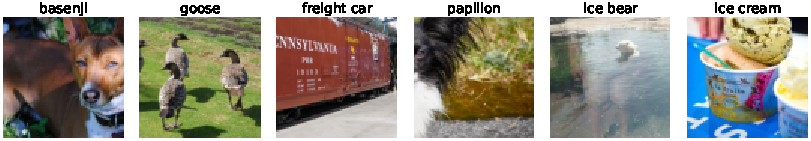
\includegraphics[width=\linewidth]{figures/eda_samples.pdf}\\[2pt]
  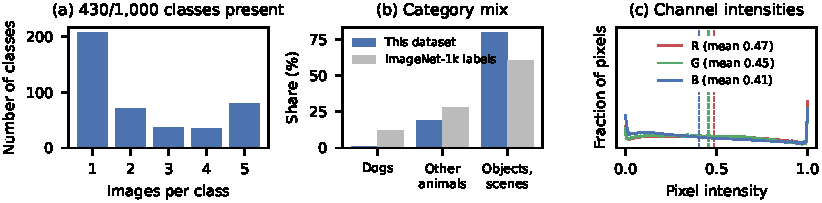
\includegraphics[width=\linewidth]{figures/eda_stats.pdf}
  \caption{Exploratory analysis. Top: random samples with their ImageNet class names (dog breed, other animal, object, repeated). (a) Only 430 of the 1,000 classes appear, each with at most five images. (b) Objects and scenes are over-represented and dog breeds under-represented relative to the ImageNet label space. (c) Per-channel pixel intensities; dashed lines mark the ImageNet normalization means, and the spikes at 0 and 1 are saturated pixels.}
  \label{fig:eda}
\end{figure}

\textbf{Exploratory analysis} (Fig.~\ref{fig:eda}). All images are $299\times299$ RGB, with no exact duplicates. \emph{Coverage:} only 430 of the 1,000 classes appear, 207 of them exactly once and none more than five times, so we analyze results per image rather than per class. \emph{Category mix:} objects and scenes make up 79.6\% of images versus 60.2\% of the label space, and dog breeds only 1.1\% versus 11.8\%, so our conclusions will mainly reflect object categories. \emph{Pixels:} channel means (0.47, 0.45, 0.41) match ImageNet's normalization constants, but the photos have more contrast (standard deviation $\approx$0.28 versus 0.23), and 2.5\% of channel values are saturated at 0 or 255, where an $L_\infty$ perturbation can move in only one direction.

\textbf{Key challenges.} (1) \emph{Label offset:} labels use the 1001-class Inception convention (0 is ``background''), so the ImageNet class is the stored label minus one, which we verified on samples (label 560 is ``folding chair''); an off-by-one error would silently corrupt every result. (2) \emph{Resolution:} images are $299\times299$ while most models expect $224\times224$, so we craft perturbations at native size and resize differentiably inside each model's wrapper. (3) \emph{Correctly classified subset:} fooling rates count only images a target gets right when clean, which differs by model, so we measure clean accuracy first. (4) \emph{Small size:} 1,000 images keep hundreds of attacks affordable but make estimates noisy, so we report bootstrap intervals.

\section{Related Work}

\textbf{Ensemble attacks.} \citet{liu2017delving} showed that adversarial examples crafted on an equal-weight ensemble transfer far better than single-model ones; this is our baseline. \citet{dong2018boosting} added momentum to iterative attacks (MI-FGSM) and found that fusing the surrogates' logits works best; we adopt this as our attack. \citet{xiong2022svre} (SVRE) reduce the variance among surrogates' gradients, and \citet{chen2023adaea} (AdaEA) adaptively reweight CNN and ViT surrogates at each step; both change \emph{how} a fixed set is combined, whereas we ask \emph{which} surrogates matter. \citet{mahmood2021robustness} found that adversarial examples rarely transfer between CNNs and ViTs, which motivates our cross-family pool and stress test.

\textbf{Shapley values and explanations.} \citet{shapley1953value} defined the unique payoff allocation satisfying efficiency, symmetry, dummy, and additivity. SHAP \citep{lundberg2017unified} uses it to attribute predictions to input features, and Data Shapley \citep{ghorbani2019data} to value individual training points; we use it to value models instead. \citet{grabisch1999axiomatic} defined the Shapley interaction index, which we use for pairs.

\textbf{Closest work.} SEAA \citep{wang2024seaa} computes Shapley values of four CNN surrogates at every attack step to reweight them, using the one-step loss increase on a rotating \emph{surrogate} as the payoff, which measures fit to the ensemble rather than transfer. We instead use success on \emph{held-out} targets as the payoff, treat the Shapley values as the finding, span three architecture families, and add pairwise interactions.

\section{Proposed Approach}

\subsection{Shared setup (both members)}

\textbf{Attack.} We study untargeted $L_\infty$ attacks with budget $\epsilon=16/255$ against a black-box target. For an ensemble $S$ with logits $z_i$, MI-FGSM \citep{dong2018boosting} increases the fused-logit loss $\mathcal{L}(x)=\mathrm{CE}\big(\frac{1}{|S|}\sum_{i\in S} z_i(x),\, y\big)$ by iterating
\begin{equation*}
  g_{k+1} = \mu\, g_k + \frac{\nabla_x \mathcal{L}(x_k)}{\lVert \nabla_x \mathcal{L}(x_k) \rVert_1},\qquad
  x_{k+1} = \Pi_{\epsilon}\big(x_k + \alpha\, \mathrm{sign}(g_{k+1})\big),
\end{equation*}
with $T=10$ iterations, step $\alpha=\epsilon/T$, and momentum $\mu=1$, where $\Pi_\epsilon$ projects onto the $\epsilon$-ball and the valid pixel range. This is the iterative FGSM (PGD) attack from Lecture~8, with two additions: a momentum term, and gradients taken through several surrogates at once, i.e., the lecture's ``ensemble of models'' transfer attack.

\textbf{Models and metric.} We use pretrained ImageNet classifiers from \texttt{timm} \citep{wightman2019timm}, each wrapped with differentiable resizing and its own normalization; Table~\ref{tab:models} lists a tentative pool. The fooling rate $\mathrm{FR}_t$ on target $t$ is the fraction of images, among those $t$ classifies correctly when clean, that it misclassifies after the attack. The targets stand in for the unseen black box: they are never used to build an attack, only to score it. We estimate on the order of ten GPU-hours on Yale's YCRC cluster.

\begin{table}[h]
  \caption{Tentative model pool. Targets are never used as surrogates.}
  \label{tab:models}
  \centering
  \small
  \setlength{\tabcolsep}{5pt}
  \begin{tabular}{lll}
    \toprule
    Family & Surrogates (8) & Held-out targets (6) \\
    \midrule
    CNN & ResNet-50, VGG-16, DenseNet-121, Inception-v3 & ResNet-152, EfficientNet-B0, ConvNeXt-T \\
    ViT & ViT-B/16, DeiT-S, Swin-T & PiT-S, BEiT-B \\
    MLP & MLP-Mixer-B/16 & ResMLP-S12 \\
    \bottomrule
  \end{tabular}
\end{table}

\subsection{Direction A (Mo Liu): Shapley valuation of surrogates}

\textbf{The game.} The players are the $n=8$ surrogates $N$. For target $t$, a coalition $S\subseteq N$ earns $v_t(S)=\mathrm{FR}_t$ of the attack crafted on $S$, with $v_t(\emptyset)=0$ because clean images are correctly classified by construction. Surrogate $i$'s Shapley value is its average marginal contribution,
\begin{equation*}
  \phi_i(v_t) = \sum_{S\subseteq N\setminus\{i\}} \frac{|S|!\,(n-|S|-1)!}{n!}\,\big[v_t(S\cup\{i\}) - v_t(S)\big],
\end{equation*}
and the Shapley interaction index $I_{ij}$ \citep{grabisch1999axiomatic} averages $v_t(S\cup\{i,j\})-v_t(S\cup\{i\})-v_t(S\cup\{j\})+v_t(S)$ over coalitions in the same way; it is positive for complementary pairs and negative for redundant ones.

\textbf{Computation.} Eight surrogates give 255 non-empty coalitions. We attack once per coalition and evaluate every result on all six targets, so one table of fooling rates yields every game exactly; this reuse is what keeps 255 attacks affordable, our main practical challenge.

\textbf{Analysis.} For each target, and averaged within each target family, we rank the surrogates by Shapley value, identify the most complementary and most redundant pairs, and compare the Shapley ranking with a ranking by standalone transfer $v_t(\{i\})$ to test our hypothesis.

\subsection{Direction B (Connor Kilrain) and synthesis}

\connor{one paragraph on your direction: question, factor or method studied, how it uses the shared pool and attack, expected output.} \textbf{Synthesis.} Because both directions share the model pool, attack, and fooling-rate table, their results are directly comparable; in the final report we will test whether the factors studied in Direction B explain the Shapley values from Direction A.

\section{Evaluation Metrics}

\textbf{Performance.} Our main metric is the fooling rate on each held-out target, for each single surrogate and for the equal-weight ensemble of all eight (the baseline), by target family. \emph{Uncertainty:} bootstrapping over images (no new attacks) gives 95\% intervals for fooling rates, Shapley values, and interactions.

\textbf{Sanity checks.} \emph{Efficiency:} the values must sum to the full ensemble's fooling rate, $\sum_i\phi_i(v_t)=v_t(N)$, to numerical precision. \emph{Dummy player:} in a five-player sub-game (four surrogates plus a randomly initialized network), the untrained network should receive credit indistinguishable from zero.

\textbf{Comparison with standalone strength.} We report the Spearman correlation $\rho$ between surrogates' Shapley values and their standalone fooling rates over the 48 surrogate--target pairs; a low $\rho$ supports our hypothesis. \textbf{Stress test.} For each target family, we restrict the game to surrogates from \emph{other} families (e.g., no ViT surrogates against PiT-S and BEiT-B), a sub-table that needs no new attacks, and check how credit shifts. \textbf{Visualization:} Shapley bar charts per target and an $8\times8$ interaction heatmap.

\textbf{Success criteria (Direction A).} (1) Efficiency holds to numerical precision and the dummy's credit is below one percentage point. (2) The values are precise enough to be informative: on most targets, bootstrap intervals separate the top-ranked surrogates from the bottom-ranked ones. We will report the hypothesis test whichever way it comes out. \textbf{Direction B:} \connor{metrics and success criteria for your direction.}

\section{Timeline}

\begin{center}
  \small
  \begin{tabular}{p{0.1\linewidth}p{0.72\linewidth}l}
    \toprule
    Date & Task & Owner \\
    \midrule
    Oct 28 & Data and label check, model wrappers, clean-accuracy filter, baseline attack & Both \\
    Nov 6  & All 255 coalition attacks; exact Shapley and interaction values; sanity checks & Mo \\
    Nov 13 & \textbf{Project milestone} & Both \\
    Nov 20 & Bootstrap intervals; Shapley vs.\ standalone rankings & Mo \\
    Dec 1  & Held-out-family stress test; Shapley and interaction figures & Mo \\
    \multicolumn{3}{l}{\connor{add your dates and tasks for Direction B as rows}} \\
    Dec 5  & Synthesis of both directions; draft report & Both \\
    Dec 16 & \textbf{Final report} (the Dec 10 exam week is a buffer) & Both \\
    \bottomrule
  \end{tabular}
\end{center}

\bibliographystyle{plainnat}
\bibliography{references}

\end{document}
